% REV00 Tue 04 May 2021 13:55:16 WIB
% START Tue 04 May 2021 13:55:16 WIB

\chapter{XXX}

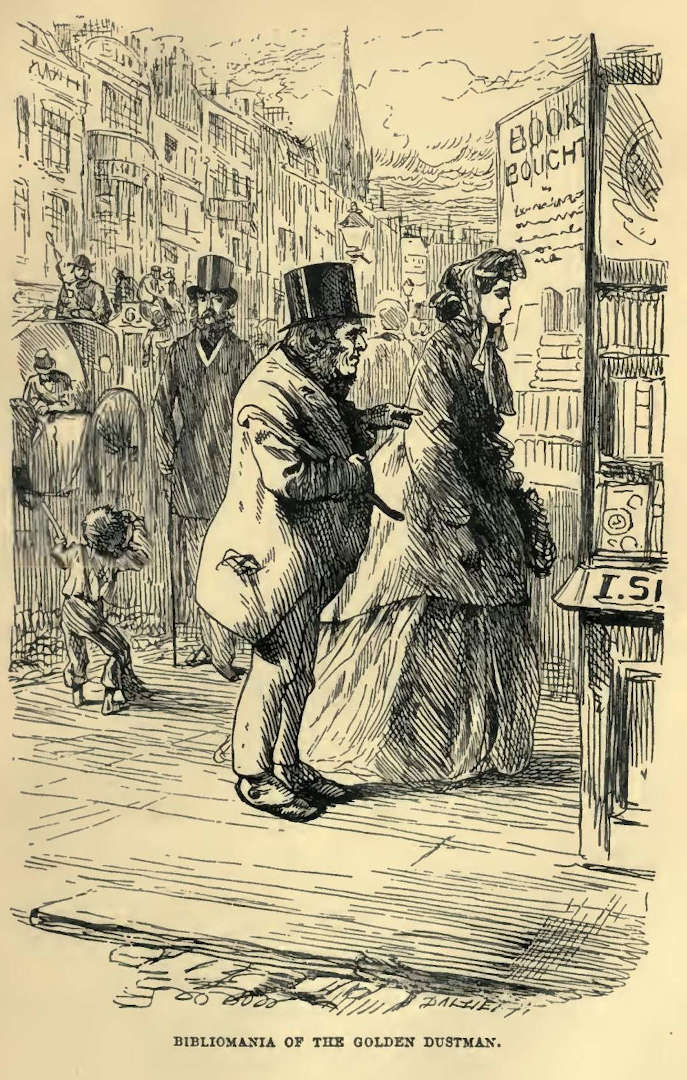
\includegraphics[scale=2.3]{03-05-01}

Chapter 8

THE END OF A LONG JOURNEY


The train of carts and horses came and went all day from dawn to
nightfall, making little or no daily impression on the heap of ashes,
though, as the days passed on, the heap was seen to be slowly melting.
My lords and gentlemen and honourable boards, when you in the course
of your dust-shovelling and cinder-raking have piled up a mountain of
pretentious failure, you must off with your honourable coats for the
removal of it, and fall to the work with the power of all the queen’s
horses and all the queen’s men, or it will come rushing down and bury us
alive.

Yes, verily, my lords and gentlemen and honourable boards, adapting your
Catechism to the occasion, and by God’s help so you must. For when we
have got things to the pass that with an enormous treasure at disposal
to relieve the poor, the best of the poor detest our mercies, hide their
heads from us, and shame us by starving to death in the midst of us, it
is a pass impossible of prosperity, impossible of continuance. It may
not be so written in the Gospel according to Podsnappery; you may not
‘find these words’ for the text of a sermon, in the Returns of the Board
of Trade; but they have been the truth since the foundations of the
universe were laid, and they will be the truth until the foundations of
the universe are shaken by the Builder. This boastful handiwork of
ours, which fails in its terrors for the professional pauper, the sturdy
breaker of windows and the rampant tearer of clothes, strikes with a
cruel and a wicked stab at the stricken sufferer, and is a horror to
the deserving and unfortunate. We must mend it, lords and gentlemen and
honourable boards, or in its own evil hour it will mar every one of us.

Old Betty Higden fared upon her pilgrimage as many ruggedly honest
creatures, women and men, fare on their toiling way along the roads
of life. Patiently to earn a spare bare living, and quietly to die,
untouched by workhouse hands--this was her highest sublunary hope.

Nothing had been heard of her at Mr Boffin’s house since she trudged
off. The weather had been hard and the roads had been bad, and her
spirit was up. A less stanch spirit might have been subdued by such
adverse influences; but the loan for her little outfit was in no part
repaid, and it had gone worse with her than she had foreseen, and she
was put upon proving her case and maintaining her independence.

Faithful soul! When she had spoken to the Secretary of that ‘deadness
that steals over me at times’, her fortitude had made too little of it.
Oftener and ever oftener, it came stealing over her; darker and ever
darker, like the shadow of advancing Death. That the shadow should
be deep as it came on, like the shadow of an actual presence, was in
accordance with the laws of the physical world, for all the Light that
shone on Betty Higden lay beyond Death.

The poor old creature had taken the upward course of the river Thames as
her general track; it was the track in which her last home lay, and of
which she had last had local love and knowledge. She had hovered for a
little while in the near neighbourhood of her abandoned dwelling, and
had sold, and knitted and sold, and gone on. In the pleasant towns of
Chertsey, Walton, Kingston, and Staines, her figure came to be quite
well known for some short weeks, and then again passed on.

She would take her stand in market-places, where there were such things,
on market days; at other times, in the busiest (that was seldom very
busy) portion of the little quiet High Street; at still other times she
would explore the outlying roads for great houses, and would ask leave
at the Lodge to pass in with her basket, and would not often get it. But
ladies in carriages would frequently make purchases from her trifling
stock, and were usually pleased with her bright eyes and her hopeful
speech. In these and her clean dress originated a fable that she was
well to do in the world: one might say, for her station, rich. As making
a comfortable provision for its subject which costs nobody anything,
this class of fable has long been popular.

In those pleasant little towns on Thames, you may hear the fall of
the water over the weirs, or even, in still weather, the rustle of the
rushes; and from the bridge you may see the young river, dimpled like a
young child, playfully gliding away among the trees, unpolluted by the
defilements that lie in wait for it on its course, and as yet out of
hearing of the deep summons of the sea. It were too much to pretend that
Betty Higden made out such thoughts; no; but she heard the tender river
whispering to many like herself, ‘Come to me, come to me! When the cruel
shame and terror you have so long fled from, most beset you, come to me!
I am the Relieving Officer appointed by eternal ordinance to do my work;
I am not held in estimation according as I shirk it. My breast is softer
than the pauper-nurse’s; death in my arms is peacefuller than among the
pauper-wards. Come to me!’

There was abundant place for gentler fancies too, in her untutored mind.
Those gentlefolks and their children inside those fine houses, could
they think, as they looked out at her, what it was to be really hungry,
really cold? Did they feel any of the wonder about her, that she felt
about them? Bless the dear laughing children! If they could have seen
sick Johnny in her arms, would they have cried for pity? If they could
have seen dead Johnny on that little bed, would they have understood it?
Bless the dear children for his sake, anyhow! So with the humbler houses
in the little street, the inner firelight shining on the panes as the
outer twilight darkened. When the families gathered in-doors there, for
the night, it was only a foolish fancy to feel as if it were a little
hard in them to close the shutter and blacken the flame. So with the
lighted shops, and speculations whether their masters and mistresses
taking tea in a perspective of back-parlour--not so far within but that
the flavour of tea and toast came out, mingled with the glow of light,
into the street--ate or drank or wore what they sold, with the greater
relish because they dealt in it. So with the churchyard on a branch of
the solitary way to the night’s sleeping-place. ‘Ah me! The dead and
I seem to have it pretty much to ourselves in the dark and in this
weather! But so much the better for all who are warmly housed at home.’
The poor soul envied no one in bitterness, and grudged no one anything.

But, the old abhorrence grew stronger on her as she grew weaker, and
it found more sustaining food than she did in her wanderings. Now, she
would light upon the shameful spectacle of some desolate creature--or
some wretched ragged groups of either sex, or of both sexes, with
children among them, huddled together like the smaller vermin for
a little warmth--lingering and lingering on a doorstep, while the
appointed evader of the public trust did his dirty office of trying to
weary them out and so get rid of them. Now, she would light upon some
poor decent person, like herself, going afoot on a pilgrimage of
many weary miles to see some worn-out relative or friend who had been
charitably clutched off to a great blank barren Union House, as far from
old home as the County Jail (the remoteness of which is always its worst
punishment for small rural offenders), and in its dietary, and in
its lodging, and in its tending of the sick, a much more penal
establishment. Sometimes she would hear a newspaper read out, and would
learn how the Registrar General cast up the units that had within the
last week died of want and of exposure to the weather: for which that
Recording Angel seemed to have a regular fixed place in his sum, as if
they were its halfpence. All such things she would hear discussed, as
we, my lords and gentlemen and honourable boards, in our unapproachable
magnificence never hear them, and from all such things she would fly
with the wings of raging Despair.

This is not to be received as a figure of speech. Old Betty Higden
however tired, however footsore, would start up and be driven away
by her awakened horror of falling into the hands of Charity. It is a
remarkable Christian improvement, to have made a pursuing Fury of the
Good Samaritan; but it was so in this case, and it is a type of many,
many, many.

Two incidents united to intensify the old unreasoning
abhorrence--granted in a previous place to be unreasoning, because the
people always are unreasoning, and invariably make a point of producing
all their smoke without fire.

One day she was sitting in a market-place on a bench outside an inn,
with her little wares for sale, when the deadness that she strove
against came over her so heavily that the scene departed from before
her eyes; when it returned, she found herself on the ground, her head
supported by some good-natured market-women, and a little crowd about
her.

‘Are you better now, mother?’ asked one of the women. ‘Do you think you
can do nicely now?’

‘Have I been ill then?’ asked old Betty.

‘You have had a faint like,’ was the answer, ‘or a fit. It ain’t that
you’ve been a-struggling, mother, but you’ve been stiff and numbed.’

‘Ah!’ said Betty, recovering her memory. ‘It’s the numbness. Yes. It
comes over me at times.’

Was it gone? the women asked her.

‘It’s gone now,’ said Betty. ‘I shall be stronger than I was afore.
Many thanks to ye, my dears, and when you come to be as old as I am, may
others do as much for you!’

They assisted her to rise, but she could not stand yet, and they
supported her when she sat down again upon the bench.

‘My head’s a bit light, and my feet are a bit heavy,’ said old Betty,
leaning her face drowsily on the breast of the woman who had spoken
before. ‘They’ll both come nat’ral in a minute. There’s nothing more the
matter.’

‘Ask her,’ said some farmers standing by, who had come out from their
market-dinner, ‘who belongs to her.’

‘Are there any folks belonging to you, mother?’ said the woman.

‘Yes sure,’ answered Betty. ‘I heerd the gentleman say it, but I
couldn’t answer quick enough. There’s plenty belonging to me. Don’t ye
fear for me, my dear.’

‘But are any of ‘em near here?’ said the men’s voices; the women’s
voices chiming in when it was said, and prolonging the strain.

‘Quite near enough,’ said Betty, rousing herself. ‘Don’t ye be afeard
for me, neighbours.’

‘But you are not fit to travel. Where are you going?’ was the next
compassionate chorus she heard.

‘I’m a going to London when I’ve sold out all,’ said Betty, rising with
difficulty. ‘I’ve right good friends in London. I want for nothing. I
shall come to no harm. Thankye. Don’t ye be afeard for me.’

A well-meaning bystander, yellow-legginged and purple-faced, said
hoarsely over his red comforter, as she rose to her feet, that she
‘oughtn’t to be let to go’.

‘For the Lord’s love don’t meddle with me!’ cried old Betty, all her
fears crowding on her. ‘I am quite well now, and I must go this minute.’

She caught up her basket as she spoke and was making an unsteady rush
away from them, when the same bystander checked her with his hand on
her sleeve, and urged her to come with him and see the parish-doctor.
Strengthening herself by the utmost exercise of her resolution, the poor
trembling creature shook him off, almost fiercely, and took to flight.
Nor did she feel safe until she had set a mile or two of by-road between
herself and the marketplace, and had crept into a copse, like a hunted
animal, to hide and recover breath. Not until then for the first time
did she venture to recall how she had looked over her shoulder before
turning out of the town, and had seen the sign of the White Lion hanging
across the road, and the fluttering market booths, and the old grey
church, and the little crowd gazing after her but not attempting to
follow her.

The second frightening incident was this. She had been again as bad, and
had been for some days better, and was travelling along by a part of
the road where it touched the river, and in wet seasons was so often
overflowed by it that there were tall white posts set up to mark the
way. A barge was being towed towards her, and she sat down on the bank
to rest and watch it. As the tow-rope was slackened by a turn of the
stream and dipped into the water, such a confusion stole into her
mind that she thought she saw the forms of her dead children and dead
grandchildren peopling the barge, and waving their hands to her in
solemn measure; then, as the rope tightened and came up, dropping
diamonds, it seemed to vibrate into two parallel ropes and strike her,
with a twang, though it was far off. When she looked again, there was no
barge, no river, no daylight, and a man whom she had never before seen
held a candle close to her face.

‘Now, Missis,’ said he; ‘where did you come from and where are you going
to?’

The poor soul confusedly asked the counter-question where she was?

‘I am the Lock,’ said the man.

‘The Lock?’

‘I am the Deputy Lock, on job, and this is the Lock-house. (Lock or
Deputy Lock, it’s all one, while the t’other man’s in the hospital.)
What’s your Parish?’

‘Parish!’ She was up from the truckle-bed directly, wildly feeling about
her for her basket, and gazing at him in affright.

‘You’ll be asked the question down town,’ said the man. ‘They won’t let
you be more than a Casual there. They’ll pass you on to your settlement,
Missis, with all speed. You’re not in a state to be let come upon
strange parishes ‘ceptin as a Casual.’

‘’Twas the deadness again!’ murmured Betty Higden, with her hand to her
head.

‘It was the deadness, there’s not a doubt about it,’ returned the man.
‘I should have thought the deadness was a mild word for it, if it had
been named to me when we brought you in. Have you got any friends,
Missis?’

‘The best of friends, Master.’

‘I should recommend your looking ‘em up if you consider ‘em game to do
anything for you,’ said the Deputy Lock. ‘Have you got any money?’

‘Just a morsel of money, sir.’

‘Do you want to keep it?’

‘Sure I do!’

‘Well, you know,’ said the Deputy Lock, shrugging his shoulders with his
hands in his pockets, and shaking his head in a sulkily ominous manner,
‘the parish authorities down town will have it out of you, if you go on,
you may take your Alfred David.’

‘Then I’ll not go on.’

‘They’ll make you pay, as fur as your money will go,’ pursued the
Deputy, ‘for your relief as a Casual and for your being passed to your
Parish.’

‘Thank ye kindly, Master, for your warning, thank ye for your shelter,
and good night.’

‘Stop a bit,’ said the Deputy, striking in between her and the door.
‘Why are you all of a shake, and what’s your hurry, Missis?’

‘Oh, Master, Master,’ returned Betty Higden, ‘I’ve fought against the
Parish and fled from it, all my life, and I want to die free of it!’

‘I don’t know,’ said the Deputy, with deliberation, ‘as I ought to let
you go. I’m a honest man as gets my living by the sweat of my brow, and
I may fall into trouble by letting you go. I’ve fell into trouble afore
now, by George, and I know what it is, and it’s made me careful. You
might be took with your deadness again, half a mile off--or half of half
a quarter, for the matter of that--and then it would be asked, Why did
that there honest Deputy Lock, let her go, instead of putting her safe
with the Parish? That’s what a man of his character ought to have done,
it would be argueyfied,’ said the Deputy Lock, cunningly harping on the
strong string of her terror; ‘he ought to have handed her over safe to
the Parish. That was to be expected of a man of his merits.’

As he stood in the doorway, the poor old careworn wayworn woman burst
into tears, and clasped her hands, as if in a very agony she prayed to
him.

‘As I’ve told you, Master, I’ve the best of friends. This letter will
show how true I spoke, and they will be thankful for me.’

The Deputy Lock opened the letter with a grave face, which underwent no
change as he eyed its contents. But it might have done, if he could have
read them.

‘What amount of small change, Missis,’ he said, with an abstracted air,
after a little meditation, ‘might you call a morsel of money?’

Hurriedly emptying her pocket, old Betty laid down on the table, a
shilling, and two sixpenny pieces, and a few pence.

‘If I was to let you go instead of handing you over safe to the Parish,’
said the Deputy, counting the money with his eyes, ‘might it be your own
free wish to leave that there behind you?’

‘Take it, Master, take it, and welcome and thankful!’

‘I’m a man,’ said the Deputy, giving her back the letter, and pocketing
the coins, one by one, ‘as earns his living by the sweat of his brow;’
here he drew his sleeve across his forehead, as if this particular
portion of his humble gains were the result of sheer hard labour and
virtuous industry; ‘and I won’t stand in your way. Go where you like.’

She was gone out of the Lock-house as soon as he gave her this
permission, and her tottering steps were on the road again. But, afraid
to go back and afraid to go forward; seeing what she fled from, in the
sky-glare of the lights of the little town before her, and leaving a
confused horror of it everywhere behind her, as if she had escaped it
in every stone of every market-place; she struck off by side ways, among
which she got bewildered and lost. That night she took refuge from the
Samaritan in his latest accredited form, under a farmer’s rick; and
if--worth thinking of, perhaps, my fellow-Christians--the Samaritan had
in the lonely night, ‘passed by on the other side’, she would have most
devoutly thanked High Heaven for her escape from him.

The morning found her afoot again, but fast declining as to the
clearness of her thoughts, though not as to the steadiness of her
purpose. Comprehending that her strength was quitting her, and that the
struggle of her life was almost ended, she could neither reason out the
means of getting back to her protectors, nor even form the idea. The
overmastering dread, and the proud stubborn resolution it engendered
in her to die undegraded, were the two distinct impressions left in her
failing mind. Supported only by a sense that she was bent on conquering
in her life-long fight, she went on.

The time was come, now, when the wants of this little life were passing
away from her. She could not have swallowed food, though a table had
been spread for her in the next field. The day was cold and wet, but
she scarcely knew it. She crept on, poor soul, like a criminal afraid of
being taken, and felt little beyond the terror of falling down while it
was yet daylight, and being found alive. She had no fear that she would
live through another night.

Sewn in the breast of her gown, the money to pay for her burial was
still intact. If she could wear through the day, and then lie down to
die under cover of the darkness, she would die independent. If she were
captured previously, the money would be taken from her as a pauper who
had no right to it, and she would be carried to the accursed workhouse.
Gaining her end, the letter would be found in her breast, along with
the money, and the gentlefolks would say when it was given back to them,
‘She prized it, did old Betty Higden; she was true to it; and while she
lived, she would never let it be disgraced by falling into the hands
of those that she held in horror.’ Most illogical, inconsequential, and
light-headed, this; but travellers in the valley of the shadow of death
are apt to be light-headed; and worn-out old people of low estate have
a trick of reasoning as indifferently as they live, and doubtless
would appreciate our Poor Law more philosophically on an income of ten
thousand a year.

So, keeping to byways, and shunning human approach, this troublesome
old woman hid herself, and fared on all through the dreary day. Yet so
unlike was she to vagrant hiders in general, that sometimes, as the day
advanced, there was a bright fire in her eyes, and a quicker beating at
her feeble heart, as though she said exultingly, ‘The Lord will see me
through it!’

By what visionary hands she was led along upon that journey of escape
from the Samaritan; by what voices, hushed in the grave, she seemed
to be addressed; how she fancied the dead child in her arms again, and
times innumerable adjusted her shawl to keep it warm; what infinite
variety of forms of tower and roof and steeple the trees took; how many
furious horsemen rode at her, crying, ‘There she goes! Stop! Stop,
Betty Higden!’ and melted away as they came close; be these things left
untold. Faring on and hiding, hiding and faring on, the poor harmless
creature, as though she were a Murderess and the whole country were up
after her, wore out the day, and gained the night.

‘Water-meadows, or such like,’ she had sometimes murmured, on the day’s
pilgrimage, when she had raised her head and taken any note of the real
objects about her. There now arose in the darkness, a great building,
full of lighted windows. Smoke was issuing from a high chimney in
the rear of it, and there was the sound of a water-wheel at the side.
Between her and the building, lay a piece of water, in which the lighted
windows were reflected, and on its nearest margin was a plantation of
trees. ‘I humbly thank the Power and the Glory,’ said Betty Higden,
holding up her withered hands, ‘that I have come to my journey’s end!’

She crept among the trees to the trunk of a tree whence she could see,
beyond some intervening trees and branches, the lighted windows, both in
their reality and their reflection in the water. She placed her orderly
little basket at her side, and sank upon the ground, supporting herself
against the tree. It brought to her mind the foot of the Cross, and
she committed herself to Him who died upon it. Her strength held out to
enable her to arrange the letter in her breast, so as that it could
be seen that she had a paper there. It had held out for this, and it
departed when this was done.

‘I am safe here,’ was her last benumbed thought. ‘When I am found dead
at the foot of the Cross, it will be by some of my own sort; some of
the working people who work among the lights yonder. I cannot see the
lighted windows now, but they are there. I am thankful for all!’


The darkness gone, and a face bending down.

‘It cannot be the boofer lady?’

‘I don’t understand what you say. Let me wet your lips again with this
brandy. I have been away to fetch it. Did you think that I was long
gone?’

It is as the face of a woman, shaded by a quantity of rich dark hair.
It is the earnest face of a woman who is young and handsome. But all is
over with me on earth, and this must be an Angel.

‘Have I been long dead?’

‘I don’t understand what you say. Let me wet your lips again. I hurried
all I could, and brought no one back with me, lest you should die of the
shock of strangers.’

‘Am I not dead?’

‘I cannot understand what you say. Your voice is so low and broken that
I cannot hear you. Do you hear me?’

‘Yes.’

‘Do you mean Yes?’

‘Yes.’

‘I was coming from my work just now, along the path outside (I was up
with the night-hands last night), and I heard a groan, and found you
lying here.’

‘What work, deary?’

‘Did you ask what work? At the paper-mill.’

‘Where is it?’

‘Your face is turned up to the sky, and you can’t see it. It is close
by. You can see my face, here, between you and the sky?’

‘Yes.’

‘Dare I lift you?’

‘Not yet.’

‘Not even lift your head to get it on my arm? I will do it by very
gentle degrees. You shall hardly feel it.’

‘Not yet. Paper. Letter.’

‘This paper in your breast?’

‘Bless ye!’

‘Let me wet your lips again. Am I to open it? To read it?’

‘Bless ye!’

She reads it with surprise, and looks down with a new expression and an
added interest on the motionless face she kneels beside.

‘I know these names. I have heard them often.’

‘Will you send it, my dear?’

‘I cannot understand you. Let me wet your lips again, and your forehead.
There. O poor thing, poor thing!’ These words through her fast-dropping
tears. ‘What was it that you asked me? Wait till I bring my ear quite
close.’

‘Will you send it, my dear?’

‘Will I send it to the writers? Is that your wish? Yes, certainly.’

‘You’ll not give it up to any one but them?’

‘No.’

‘As you must grow old in time, and come to your dying hour, my dear,
you’ll not give it up to any one but them?’

‘No. Most solemnly.’

‘Never to the Parish!’ with a convulsed struggle.

‘No. Most solemnly.’

‘Nor let the Parish touch me, not yet so much as look at me!’ with
another struggle.

‘No. Faithfully.’

A look of thankfulness and triumph lights the worn old face.

The eyes, which have been darkly fixed upon the sky, turn with meaning
in them towards the compassionate face from which the tears are
dropping, and a smile is on the aged lips as they ask:

‘What is your name, my dear?’

‘My name is Lizzie Hexam.’

‘I must be sore disfigured. Are you afraid to kiss me?’

The answer is, the ready pressure of her lips upon the cold but smiling
mouth.

‘Bless ye! NOW lift me, my love.’

Lizzie Hexam very softly raised the weather-stained grey head, and
lifted her as high as Heaven.



